\documentclass[border=4pt]{standalone}
\usepackage[T1]{fontenc}
\usepackage{helvet}
\renewcommand{\familydefault}{\sfdefault}
\usepackage{graphicx}
\usepackage{caption}
\usepackage{amsmath}
\captionsetup{font={sf,footnotesize},labelfont={sf,bf,footnotesize},justification=justified,singlelinecheck=false}
\begin{document}
\begin{minipage}{7.20in}
\centering
\begin{figure}[htbp]
    \centering
    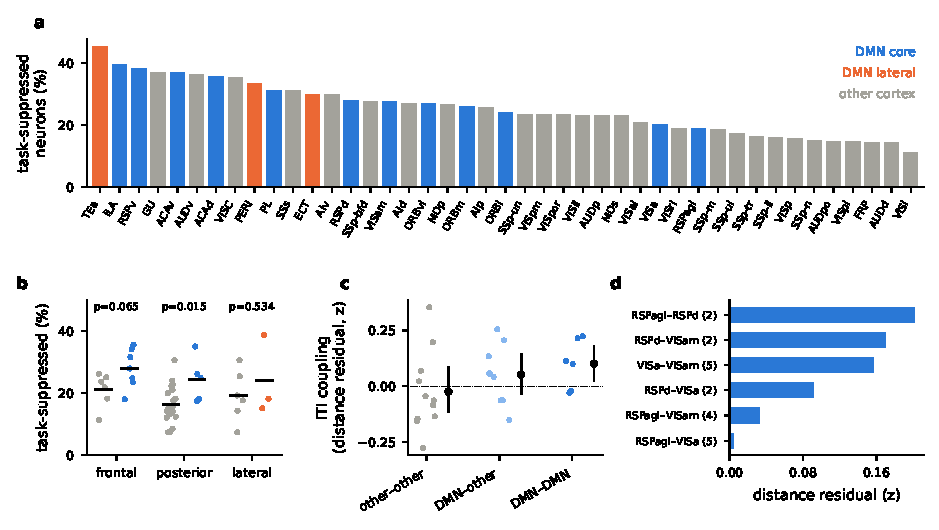
\includegraphics[width=\linewidth]{fig_dmn_panels.pdf}
    \caption{\textbf{a} BWM Neuropixels, 419 sessions, 137 mice: percentage of neurons per cortical region (Beryl) significantly suppressed during the task (stimulus, movement and feedback windows) relative to still inter-trial rest. Blue, DMN core (ACA, PL, ILA, ORB, RSP, VISa, VISam); orange, DMN lateral (TEa, ECT, PERI); grey, other cortex. \textbf{b} Same measure under strict stillness, DMN regions vs non-DMN neighbours within frontal (vs MOs, MOp, FRP, AI), posterior (vs SSp, AUD, VIS) and lateral (vs AUD, VISC, GU) cortex; dots are regions, bars means, region-permutation p. \textbf{c} Mesoscope (45 sessions, 11 mice): correlation of region-averaged calcium activity in still inter-trial bins (1 s, wheel/lick/motion-energy regressed), as residual from the distance-matched mean; dots are mice, black mean and 95\% mouse-bootstrap CI. \textbf{d} Mean residual coupling per DMN region pair (number of mice in brackets); the DMN--DMN excess is carried by VISa--VISam and RSP pairs.}
    \label{fig:dmn}
\end{figure}
\end{minipage}
\end{document}
